\documentclass[letterpaper, 12 pt, conference]{ieeeconf}

\IEEEoverridecommandlockouts
% This command is only needed if 
% you want to use the \thanks command

\overrideIEEEmargins
% Needed to meet printer requirements.
%\usepackage[margin=0.65in]{geometry}

% See the \addtolength command later in the file to balance the column lengths
% on the last page of the document

% The following packages can be found on http:\\www.ctan.org
\usepackage{graphics} % for pdf, bitmapped graphics files
\usepackage{epsfig} % for postscript graphics files
\usepackage{mathptmx} % assumes new font selection scheme installed
\usepackage{times} % assumes new font selection scheme installed
\usepackage{amsmath} % assumes amsmath package installed
\usepackage{amssymb}  % assumes amsmath package installed

\usepackage{hyperref}
\usepackage{url}
%\usepackage[pdftex]{graphicx}
%\usepackage{amsfonts}
\usepackage{subfigure} 
\usepackage{algorithm}
%\usepackage{algorithmic}
\usepackage{algcompatible}
\usepackage{framed}
\usepackage{balance}
\graphicspath{{images/}}

\title{\LARGE \bf
Generating Natural Language Descriptions of Trajectories Using Long Short Term Memory Neural Networks}

\author{Rodolfo Corona and Rolando Fernandez}

\begin{document}

\maketitle
\thispagestyle{empty}
\pagestyle{empty}

\section{Problem Description}

Given a point-cloud $p$ $\in$ $P$ and a manipulation trajectory $t$ $\in$ $T$, our goal is to output a free-form  Natural Language (NL) description $l$ $\in$ $L$ that describes the trajectory $t$:

\begin{equation}
f: T\times P \mapsto L
\end{equation}

\section{Background on LSTMs}

LSTMs are a variant of the Recurrent Neural Network (RNN) architecture which attempt to alleviate the vanishing gradient problem which traditional RNNs can suffer from. 
\par
LSTMs accomplish this through the use of \textit{gates}, which, change the cell's state at each time step based on the current time step's input and the last time step's output. Intuitively, at each time step, an LSTM cell decides which information to forget and which new information to incorporate through the use of its gates. Formally, this computation takes the form of the following gate update equations: 

\begin{align*}
f_t &= \sigma (W_fx_t + U_fh_{t-1}+b_f) \\
i_t&=\sigma (W_ix_t + U_ih_{t-1}+b_i) \\
c_t &= tanh (W_cx_t  + U_c h_{t-1}+b_c) \\
o_t &= \sigma (W_o x_t + U_o h_{t-1} + b_o)
\end{align*}

And the cell state update and output equations:

\begin{align*}
C_t &= f_tC_{t-1}+ i_t c_t \\
h_t&= o_t \cdot tanh(C_t)
\end{align*}


\section{Methods}

\subsection{Robobarista Dataset}

Sung et al. developed the Robobarista framework in order perform Deep Multimodal embedding of point clouds and NL Descriptions to Trajectories, as shown in Equation (2). Sung et al. aimed to create a system for manipulation planning which could generalize to different objects with similar parts to be manipulated \cite{sung2016robobarista}. 

\begin{equation}
f: P\times L \mapsto T
\end{equation}

Using the Robobarista framework Sung et al. collected an extensive dataset of consisting of triplets of the form (point cloud, NL Descriptions, and Trajectory). The dataset consists of 116 objects with 249 parts along with 250 NL instructions, for which there was collected 1225 manipulation trajectories. 

Each of the 116 objects is split into parts depending on the number of NL instructions that pertain to it and the original point cloud scene is segmented with respect to the part frames, being stored as a Comma Separated Value (CSV) file consisting of [x,y,z,r,g,b] values. 

Furthermore, each of the objects have multiple manipulation trajectories for each part stored as a list of waypoints \cite{sung2016robobarista}. For our experiments we split the dataset into 5 folds of train and test data in order to perform 5 fold cross validation at the end of our experiments.

\subsection{Baseline with Point Clouds}
For our initial baseline we created a pipeline that utilizes the point clouds and NL descriptions in the Robobarista dataset to perform inference using K-Means clustering and K-Nearest Neighbors (Figure \ref{fig:Baseline_Point_Cloud}). We first train a K-Means model and a KNN model using the training data for each of the 5 folds.

The point cloud key points are taken from the segmented object part point cloud CSV files. We create two vectors from the CSV files, one is a vector of all the point Clouds in the training set where the point clouds themselves are vectors of key points and the other is a vector of all the key points in the training set. 

Utilizing the K-Means algorithm in the Python SKLearn package, we input the vector of all the key points in the training set into the K-Means algorithm with a cluster count of 50 and get back trained K-Means model. With the K-Means model we extract a closest cluster prediction for the key points in each individual point cloud in the vector of all the point clouds in the training set. Then using the cluster predictions we compute a Bag of Features (BOF) vector for each point cloud based on the number of occurrences of each cluster.

The BOF vectors are then used as input with a neighbor count of 1 to the K-Nearest Neighbors classifier in the Python SKLearn package and in return we get a trained KNN model. We are then able to use this KNN model to determine the nearest neighbors of a given point cloud. 


\begin{figure}[htb!]
  \centering
  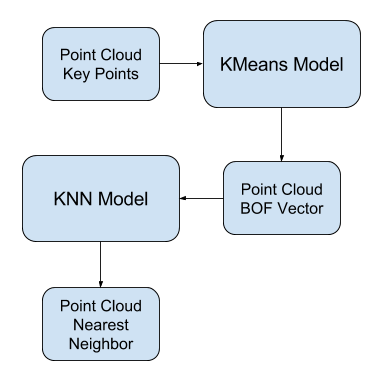
\includegraphics[width=0.3\textwidth]{Baseline-[Point_Cloud]}
  \caption{Baseline with Point Clouds}
  \label{fig:Baseline_Point_Cloud}
\end{figure}

\subsection{LSTM Implementation}

We currently implement an encoder-decoder LSTM neural network architecture. Specifically, our architecture uses one LSTM layer to encode the inputted sequence of trajectory waypoints $t$ into an embedding $h$. This embedding is then fed into another LSTM layer which decodes it into a sequence of words $y$. We use the Keras\footnote{https://keras.io/} library with a TensorFlow\footnote{https://www.tensorflow.org/} backend to implement our network architecture.   

\begin{figure}[h]
\center
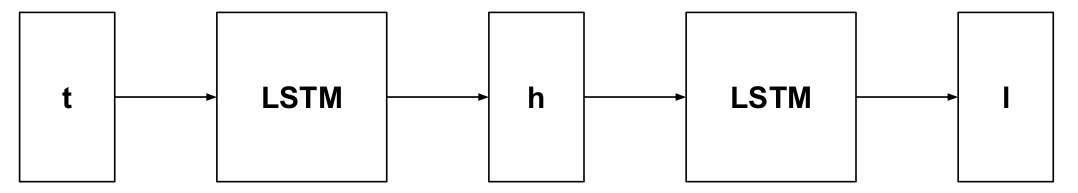
\includegraphics[scale=0.20]{Trajectory_LSTM}
\caption{Our current LSTM encoder-decoder architecture. $x_t$ represents a trajectory waypoint sequence, $h_t$ represents the embedding generated by the encoder, and $y_t$ is the word sequence generated by the decoder.}
\end{figure}

\subsection{Preprocessing}
After analyzing the Robobarista dataset, it was found  that the longest trajectory consisted of 18 waypoints. Therefore, all trajectories were fitted into tensors of 18 waypoints, with zero vectors used to pad trajectories with less than 18 waypoints. 
\par
Similarly, it was found that all phrases in the dataset consisted of less than 18 words. Each phrase was converted into a tensor consisting of 18 one-hot vectors of dimensionality $|V|$, where $|V|$ is the size of the training set vocabulary.

\subsection{Training}

Our current architecture consists of 50 hidden units in both the encoder and decoder. We have trained our network over 1000 epochs with a batch size of 80, a mean squared error loss function, and RMSProp optimizer with a learning rate of 0.001. 

\subsection{Testing}

During testing, we feed a trajectory tensor to our network which then generates a sequence of one-hot vectors for phrases. Because every phrase in our dataset ends with a "." token, we generate phrases of 18 tokens and prune them up to the first appearance of the "." token.  


\section{Results}

\subsection{Baseline with Point Clouds}

For the baseline we conducted experiments using the data from each of the 5 folds, running a total of 5 trials. For each trial we created a gold reference consisting of the already known NL descriptions for each of the point clouds and a test reference consisting of the NL description returned by using the trained K-Means and KNN models.

Each point cloud in the fold test data is first inputed in the K-Means model to extract the BOF vector representation, then the BOF vector is inputed into the KNN model to retrieve the nearest neighbor of the point cloud, and lastly we look up the NL description for the given neighbor. With the completed the test and gold reference files we are then able to use the sentence comparison package METEOR to evaluate the accuracy of the Baseline with point clouds \cite{Denkowski14meteoruniversal}.

On average the baseline performed poorly as only reaching its highest performance in the first fold achieving a final Meteor score of 0.172. Figure \ref{fig:fold_1_score}, shows the performance statistics for each sentence compared in Fold 1. Figures \ref{fig:fold_1_sentence_148} and \ref{fig:fold_1_sentence_164}, show the individual sentence comparisons results for two sentences from the Fold 1 test set. These results were expected as the Baseline only performs a simple lookup based on nearest neighbor inference and is not able to adapt properly.

\begin{figure}[htb!]
  \centering
  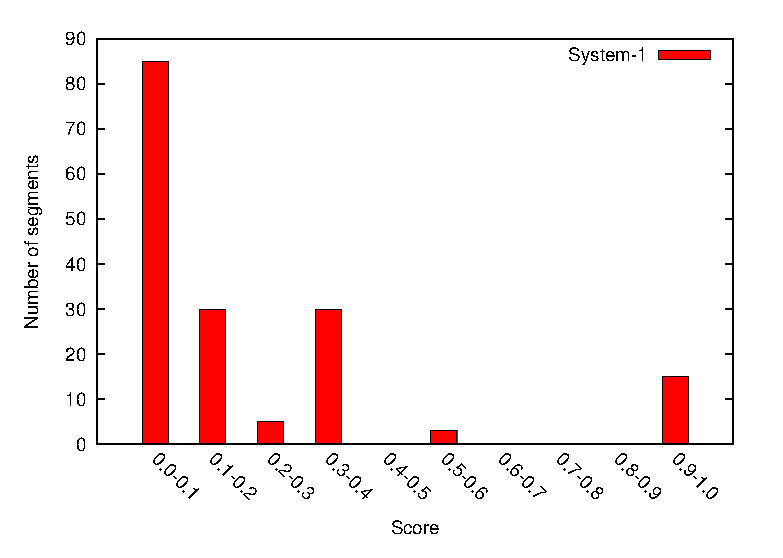
\includegraphics[width=0.45\textwidth]{fold_1_score}
  \caption{Meteor Score for Fold 1 Test Data}
  \label{fig:fold_1_score}
\end{figure}

\begin{figure}[htb!]
  \centering
  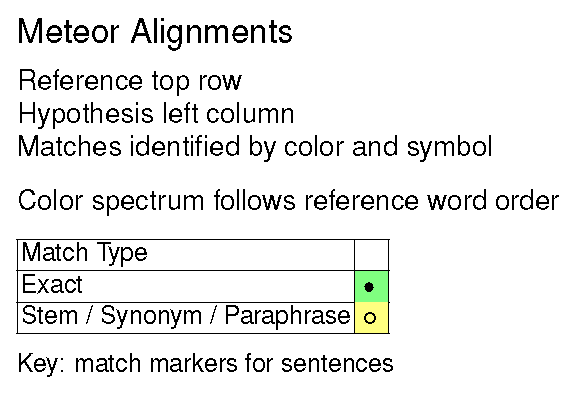
\includegraphics[width=0.45\textwidth]{meteor_alignment_key}
  \caption{Meteor Alignment Key}
  \label{fig:meteor_alignment_key}
\end{figure}

\begin{figure}[htb!]
  \centering
  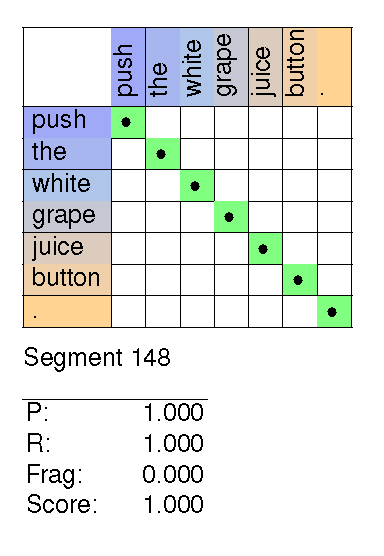
\includegraphics[width=0.3\textwidth]{fold_1_sentence_148}
  \caption{Meteor Alignment for Fold 1 Sentence 148}
  \label{fig:fold_1_sentence_148}
\end{figure}

\begin{figure}[htb!]
  \centering
  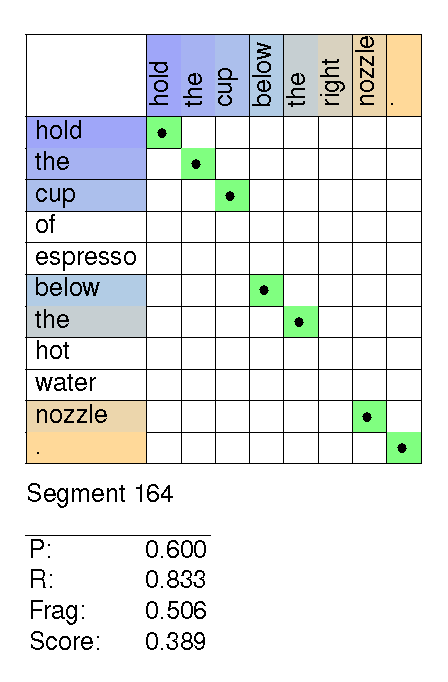
\includegraphics[width=0.3\textwidth]{fold_1_sentence_164}
  \caption{Meteor Alignment for Fold 1 Sentence 164}
  \label{fig:fold_1_sentence_164}
\end{figure}

\subsection{LSTM Implementation}

\section{Difficulties}

The major difficulty we have encountered up to this point is that we have not been able yet to receive a complete trained model for the work performed by Sung et al. \cite{sung2016robobarista}. To overcome the lack of the trained model for our Baseline experiments we decided to attempt to use Dynamic Time Warping to compare trajectories that are associated with the point clouds. 

Additionally, we discovered why developing our Baseline experiments that the segmented points clouds for each object part are not stored in the typical Point Cloud Data (PCD) format, but instead are stored in a CSV format where each point cloud point is represented as a list of values [x,y,z,r,g,b]. To deal with this unexpected format we decided to forgo the use of NARF \cite{steder2010narf} descriptors and instead consider each point in the segmented point clouds as a key point for use in the BOF comparison method using the K-Nearest Neighbors method. 

\section{Outlook}

\section{Future Work}

In addition, to the current Baseline with point clouds we propose conducting two more Baseline experiments, one using only trajectories and the other using trajectories and point clouds. For the Baseline using only trajectories it will only be possible to perform this Baseline if we are able to receive a trained model for the work by Sung et al. \cite{sung2016robobarista}. The Baseline using point clouds and trajectories we be performed by retrieving some $k$ number of neighbor point clouds and re-ranking based on the similarity of the trajectories using Dynamic Time Warping.

For the conclusion of the project, we propose to implement a two layer LSTM architecture as in \cite{Venugopalan_2015_ICCV}. Additionally, this architecture will incorporate point cloud data by concatenating the bag of feature vectors produced from a point cloud to the trajectory embedding produced by the LSTM encoding layers. Finally, we will continue to experiment with different parameters for our LSTM architecture such as through different numbers of hidden units and training epochs. 

\begin{figure}[h]
\centering
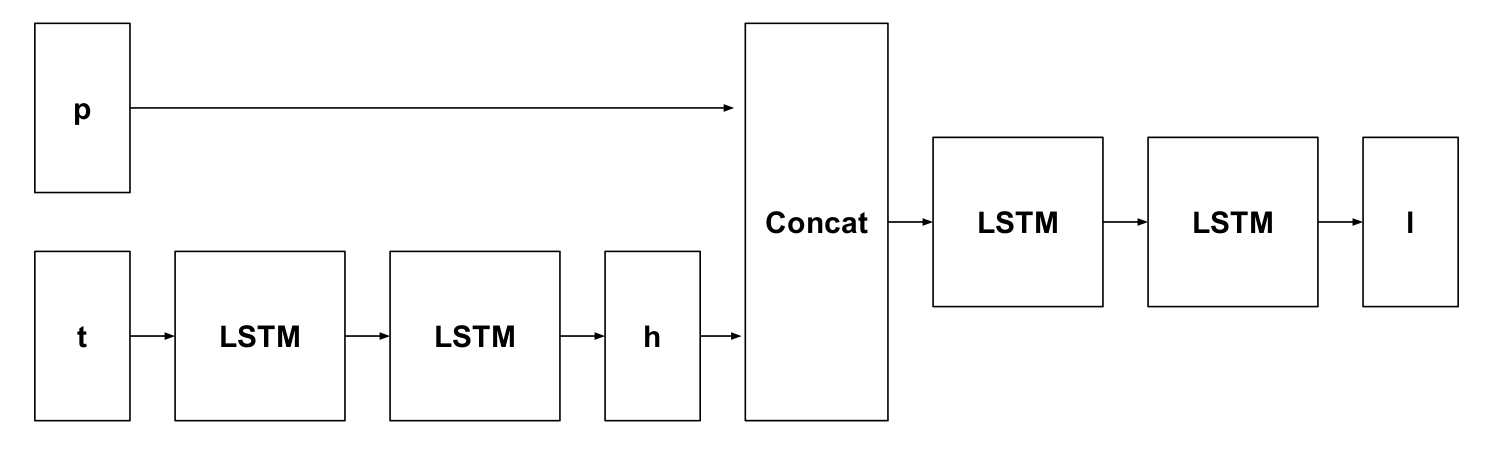
\includegraphics[scale=0.15]{Tuple_LSTM}
\caption{The proposed final architecture for our LSTM model. The network will use a double layer LSTM encoder to generate trajectory embeddings. The two layer decoder will then be trained on the concatenation between the embedding and the point cloud bag of features vector to generate word sequences.}
\end{figure}

\section{Justification of Progress}

We believe that we have made sufficient progress to put ourselves on track with the project deadlines due to the fact that we have created a full pipeline for our Baseline and LSTM experiments. To continue forward we will only have to perform some slight modifications to our models to account for the additional parameters in order to use both point clouds and trajectories.


%\bibliographystyle{abbrv}
\bibliographystyle{IEEEtran}
\bibliography{citations}

\end{document}
